%%% use twocolumn and 10pt options with the asme2ej format
\documentclass[twocolumn,10pt]{asme2ej}

\usepackage{epsfig} %% for loading postscript figures
\usepackage{subfigure}
\usepackage{titling}
\usepackage{siunitx}
\usepackage[hidelinks]{hyperref}
\usepackage{fancyhdr}
\pagestyle{fancy}
\renewcommand{\headrulewidth}{0pt}
\fancyhead{}
\fancyfoot{}
\fancyfoot[R]{\thepage}

\def\figureautorefname{Fig.} 
\def\equationautorefname{Eq.} 
\def\sectionautorefname{Sez.} 
\def\subsectionautorefname{Sez.} 
\def\subsubsectionautorefname{Sez.}


\pretitle{\begin{center}\linespread{1.2}\huge}
\posttitle{\par\end{center}\vspace{0.5em}}

\abovedisplayshortskip=0pt
\belowdisplayshortskip=0pt
\abovedisplayskip=-5pt
\belowdisplayskip=5pt


%% The class has several options
%  onecolumn/twocolumn - format for one or two columns per page
%  10pt/11pt/12pt - use 10, 11, or 12 point font
%  oneside/twoside - format for oneside/twosided printing
%  final/draft - format for final/draft copy
%  cleanfoot - take out copyright info in footer leave page number
%  cleanhead - take out the conference banner on the title page
%  titlepage/notitlepage - put in titlepage or leave out titlepage
%  
%% The default is oneside, onecolumn, 10pt, final

\date{}
\title{{\huge\bfseries Laboratorio di Fisica} - {\LARGE A.A. 2020/2021} \\ 
    {\LARGE Docenti: A. Garfagnini - M. Lunardon} \\ {\Huge\bfseries Effetto Zeeman}}


%%% first author
\author{Cerrone Vanessa
    \affiliation{
    1200361\\
    vanessa.cerrone@studenti.unipd.it
    }	
}

%%% second author
\author{Cigagna Simone
    \affiliation{
	1193992\\
    simone.cigagna@studenti.unipd.it
    }	
}

%%% third author
\author{Lai Nicolò
    \affiliation{
	1193976\\
    nicolo.lai@studenti.unipd.it
    }	
}


\begin{document}


\maketitle    


% %%%%%%%%%%%%%%%%%%%%%%%%%%%%%%%%%%%%%%%%%%%%%%%%%%%%%%%%%%%%%%%%%%%%%%
\section{Introduzione}\label{s:introduzione}

L'effetto Zeeman normale è un fenomeno fisico che consiste nella separazione delle righe di emissione di un atomo
eccitato in presenza di un campo magnetico esterno $\vec{\text{B}}$. L'interazione con il campo è riconducibile a onde
elettromagnetiche emesse da dipoli oscillanti, per cui il moto orbitale dell'elettrone può essere scomposto in un moto
oscillatorio lungo la direzione di $\vec{\text{B}}$ ($\Delta \text{m} = 0$) e un moto rotatorio destrogiro o levogiro
attorno a $\vec{\text{B}}$ ($\Delta \text{m} = \pm1$). Nell'esperienza si analizza tale effetto nell'atomo di Neon,
studiando la riga spettrale a $585.3 \,\si{\nano\metre}$ data dalla transizione $ ^1\text{S}_0 \rightarrow ^1\text{P}_1$,
cioè tra stati con spin $\text{S} = 0$ e $\Delta \text{L}= \Delta \text{J} = 1$. \\
Si utilizza lo spettrometro \textit{Zeeman 2} e come sorgente di luce una lampada al Neon a scarica a bagliore
alimentata in corrente continua: le incertezze sulle dimensioni dei componenti, in particolare della lamina di Lummer, e
degli altri dati di costruzione sono trascurabili rispetto alle incertezze statistiche, mentre l'incertezza relativa sul
valore del campo magnetico $\vec{\text{B}}$ risulta essere dell' $1\%$.   \\

Ai fini dello studio dell'effetto Zeeman, in \autoref{s:neon} verrà effettuata una breve analisi dello spettro emissivo
del Neon volta a ricercare la riga di interesse a $585.3 \,\si{\nano\metre}$. Successivamente, in \autoref{s:risolvente}
si verificherà che il potere risolvente dell'apparato sia sufficientemente alto da poter rivelare la separazione dei
livelli energetici. Tale separazione verrà poi studiata in dettaglio in \autoref{s:lande} tramite la stima del fattore
di Landè. Infine, in \autoref{s:ortogonale} verranno analizzati qualitativamente gli effetti dovuti all'orientazione del
campo magnetico esterno, sia in assenza di un filtro polarizzatore, sia in due diverse configurazioni di quest'ultimo.




% %%%%%%%%%%%%%%%%%%%%%%%%%%%%%%%%%%%%%%%%%%%%%%%%%%%%%%%%%%%%%%%%%%%%%%
\section{Spettro di emissione del Neon}\label{s:neon}

Si vuole inizialmente studiare lo spettro emissivo del Neon per individuare correttamente la riga a $585.3
\,\si{\nano\metre}$, corrispondente alla transizione di interesse.\\
Lo spettro viene acquisito con il CCD posizionato orizzontalmente, a campo magnetico spento, e in assenza della lamina
di Lummer. Per l'acquisizione dello spettro, si utilizza un tempo di integrazione pari a $100 \,\si{\milli\second}$. \\
Si effettua poi una calibrazione dell'asse orizzontale, convertendo così il numero di pixel relativi al CCD in lunghezze
d'onda. A tale scopo, si predispone una regressione lineare delle lunghezze d'onda delle principali righe spettrali del
Neon in funzione del numero di pixel corrispondenti ai picchi rivelati dal detector. 
 
\begin{figure*}
    \centering
    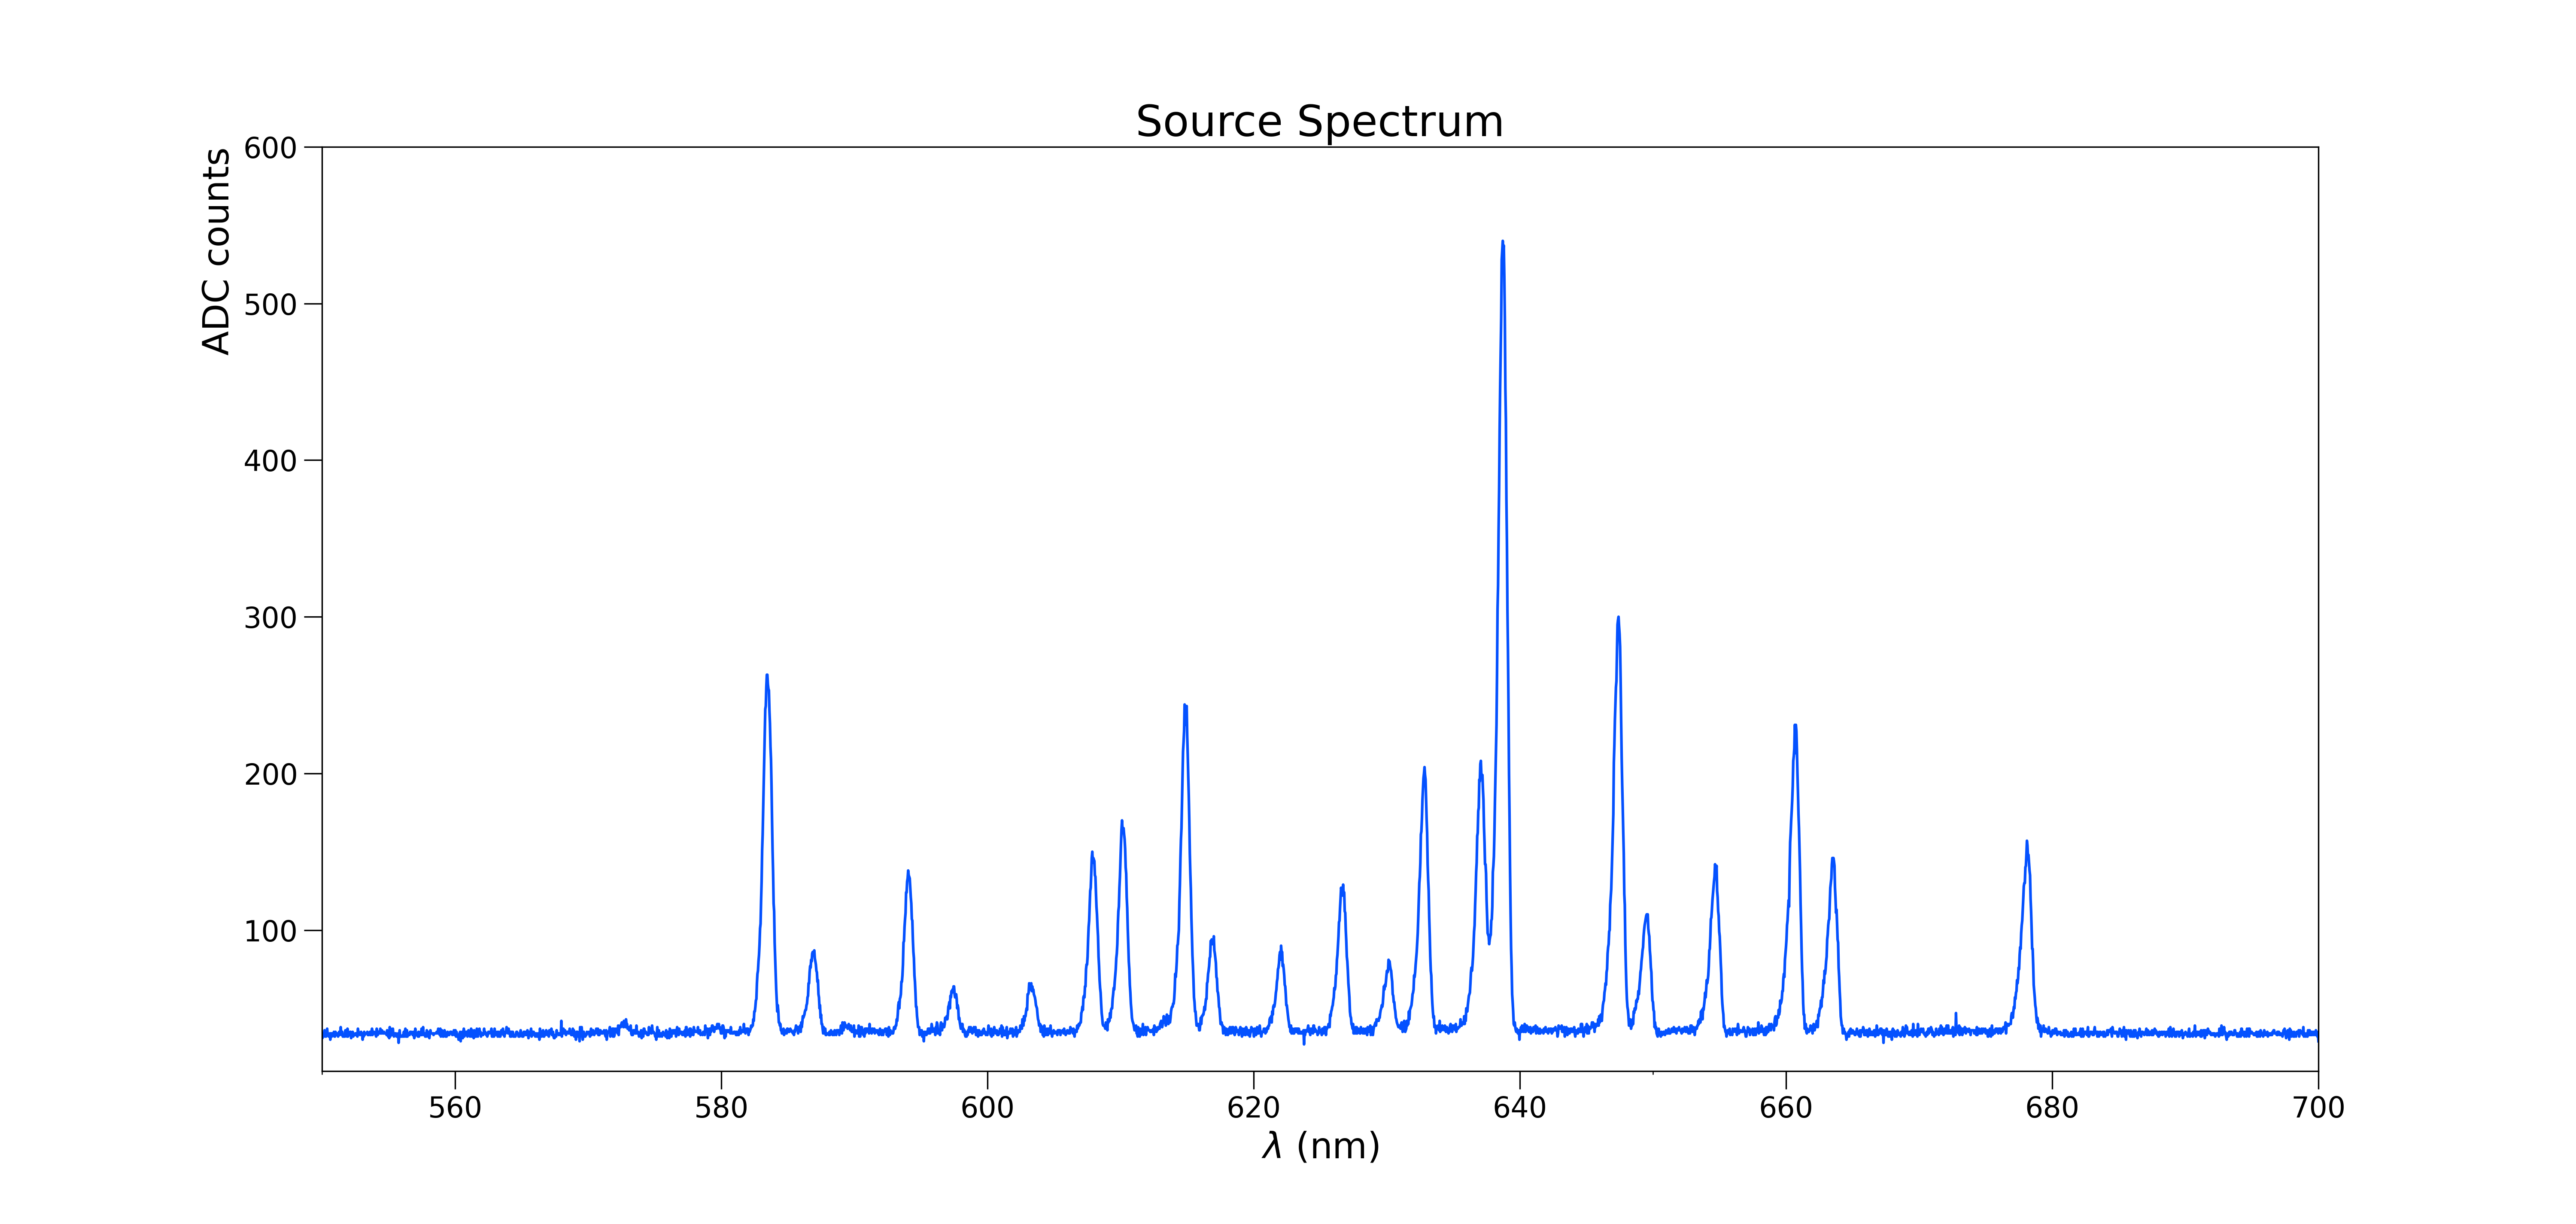
\includegraphics[width=\textwidth]{../Spectrum/SpectrumPlots/spettro1d_Boff.png}
    \caption{Spettro emissivo del Neon con asse orizzontale calibrato}
    \label{i:spettro1d}
\end{figure*}


In \figurename\ref{i:spettro1d} viene rappresentato lo spettro di emissione con l'asse orizzontale calibrato: si
osservano evidenti transizioni nella regione $580-680 \,\si{\nano\metre}$, in particolare la riga più intensa a $640.2
\,\si{\nano\metre}$ e la riga di interesse per l'esperienza a $585.3 \,\si{\nano\metre}$.\\
Si vuole far notare, infine, che in presenza di un campo magnetico esterno lo spettro rimane invariato a meno
dell'intensità della radiazione rivelata, che aumenta significativamente. 




% %%%%%%%%%%%%%%%%%%%%%%%%%%%%%%%%%%%%%%%%%%%%%%%%%%%%%%%%%%%%%%%%%%%%%%
\section{Potere risolvente dell'apparato}\label{s:risolvente}

% \begin{itemize}
%     \item Lo calcoliamo con Boff
%     \item Formule (range utile ecc ecc) (approx luce radente) 
%     \item Procedura di analisi (indipendenza statistica, picchi a triplette ecc ecc)
%     \item Plot con tutti i picchi fittati + finestrella con lo zoom su una tripletta
%     \item Stima di R (come quando perchè)
%     \item Plot del trend per aberrazione 
% \end{itemize}


Il potere risolvente R dell'apparato sperimentale si definisce come

\vspace{-15pt}
\begin{equation}
    R = \frac{\lambda}{\Delta\lambda}
    \label{e:r}
\vspace{-5pt}
\end{equation}

dove, nel caso di interesse, $\lambda = 585.3 \,\si{\nano\metre}$ e $\Delta\lambda$ corrisponde alla larghezza a metà
altezza (in nanometri) dei picchi di interferenza causati dal prisma presente nell'apparato. Per prima cosa, quindi,
sarà necessario convertire la larghezza dei picchi da pixel del CCD a nanometri: ponendosi nell'approssimazione di luce
radente vale:

\vspace{-10pt}
\begin{equation}
    \Delta\lambda_{\text{r.u.}} \simeq \frac{\lambda^2}{2\text{d}}
    \label{e:dlambdaru}
\vspace{-5pt}
\end{equation}

Tale quantità corrisponde alla distanza approssimata tra due picchi di interferenza, espressa in nanometri, e dipende
quindi sia dalla lunghezza d'onda della riga $\lambda$ sia dallo spessore della lamina di Lummer d.\\
Conoscendo quindi $\Delta\lambda_{\text{r.u.}}$ è possibile ricavare la larghezza a metà altezza, espressa in nanometri,
dei picchi di interferenza secondo

\vspace{-15pt}
\begin{equation}
    \Delta\lambda = \frac{\Delta\lambda_{\text{r.u.}}}{\Delta x_{\text{r.u.}}} \cdot \Delta x
    \label{e:dlambda}
\vspace{-5pt}
\end{equation}

dove $\Delta x_{\text{r.u.}}$ corrisponde alla distanza tra due picchi espressa in pixel e $\Delta x$ rappresenta la
larghezza a metà altezza dei picchi espressa in pixel.  \\

Si procede quindi restringendo l'intervallo di acquisizione ad un intorno della riga evidenziata in
\autoref{i:spettro1d}: viene quindi ruotato il CCD in posizione verticale e viene inserita la lamina di Lummer. Il tempo
di integrazione scelto per l'acquisizione è di $800\,\si{\milli\second}$. Si sottolinea inoltre che il campo magnetico
rimane spento. \\
Il risultato dell'acquisizione corrisponde allo spettro bidimensionale raffigurato in \autoref{i:spettro2d_Boff} (a
sinistra). A destra invece viene presentata la proiezione sull'asse orizzontale di tale istogramma. In particolare, gli
istogrammi rappresentati in \autoref{i:spettro2d_Boff} sono ottenuti sottraendo il rumore di fondo: nella figura a
sinistra, infatti, si nota chiaramente la presenza della riga di emissione. \\
Per calcolare ora le grandezze di interesse, quali la spaziatura tra picchi e la loro larghezza a metà altezza, si
considera la proiezione dello spettro sull'asse verticale, evidenziando in questo modo le frange di interferenza causate
dal prisma dell'apparato. Per evitare di ottenere un campione di misure statisticamente dipendenti di $\Delta
x_{\text{r.u.}}$ e $\Delta x$ (e di conseguenza di $\Delta\lambda$ ed R, calcolate a partire dalle prime) si sceglie di
suddividere i picchi di interferenza in triplette contigue. In questo modo, la spaziatura tra i picchi viene calcolata
come media aritmetica della distanza tra i due picchi esterni della tripletta rispetto a quello centrale. Infine, la
larghezza a metà altezza viene misurata unicamente per il picco centrale. Come si può notare in
\autoref{i:spettro2d_Boff_ProjY}, in particolare nel riquadro in alto a sinistra, tutti i picchi vengono fittati da una
funzione gaussiana: la spaziatura tra i picchi viene calcolata utilizzando il centroide delle gaussiane esterne mentre
la FWHM del picco centrale si misura a partire dal valore massimo del fit. \\
Si ottiene, così facendo, un campione di 6 misure di $\Delta x_{\text{r.u.}}$ e $\Delta x$ tra loro statisticamente
indipendenti. Si procede dunque al calcolo di $\Delta\lambda$ secondo \autoref{e:dlambda}, ottenendo infine un campione
di poteri risolventi R calcolati seguendo \autoref{e:r}. 




\begin{figure}
    \centering
    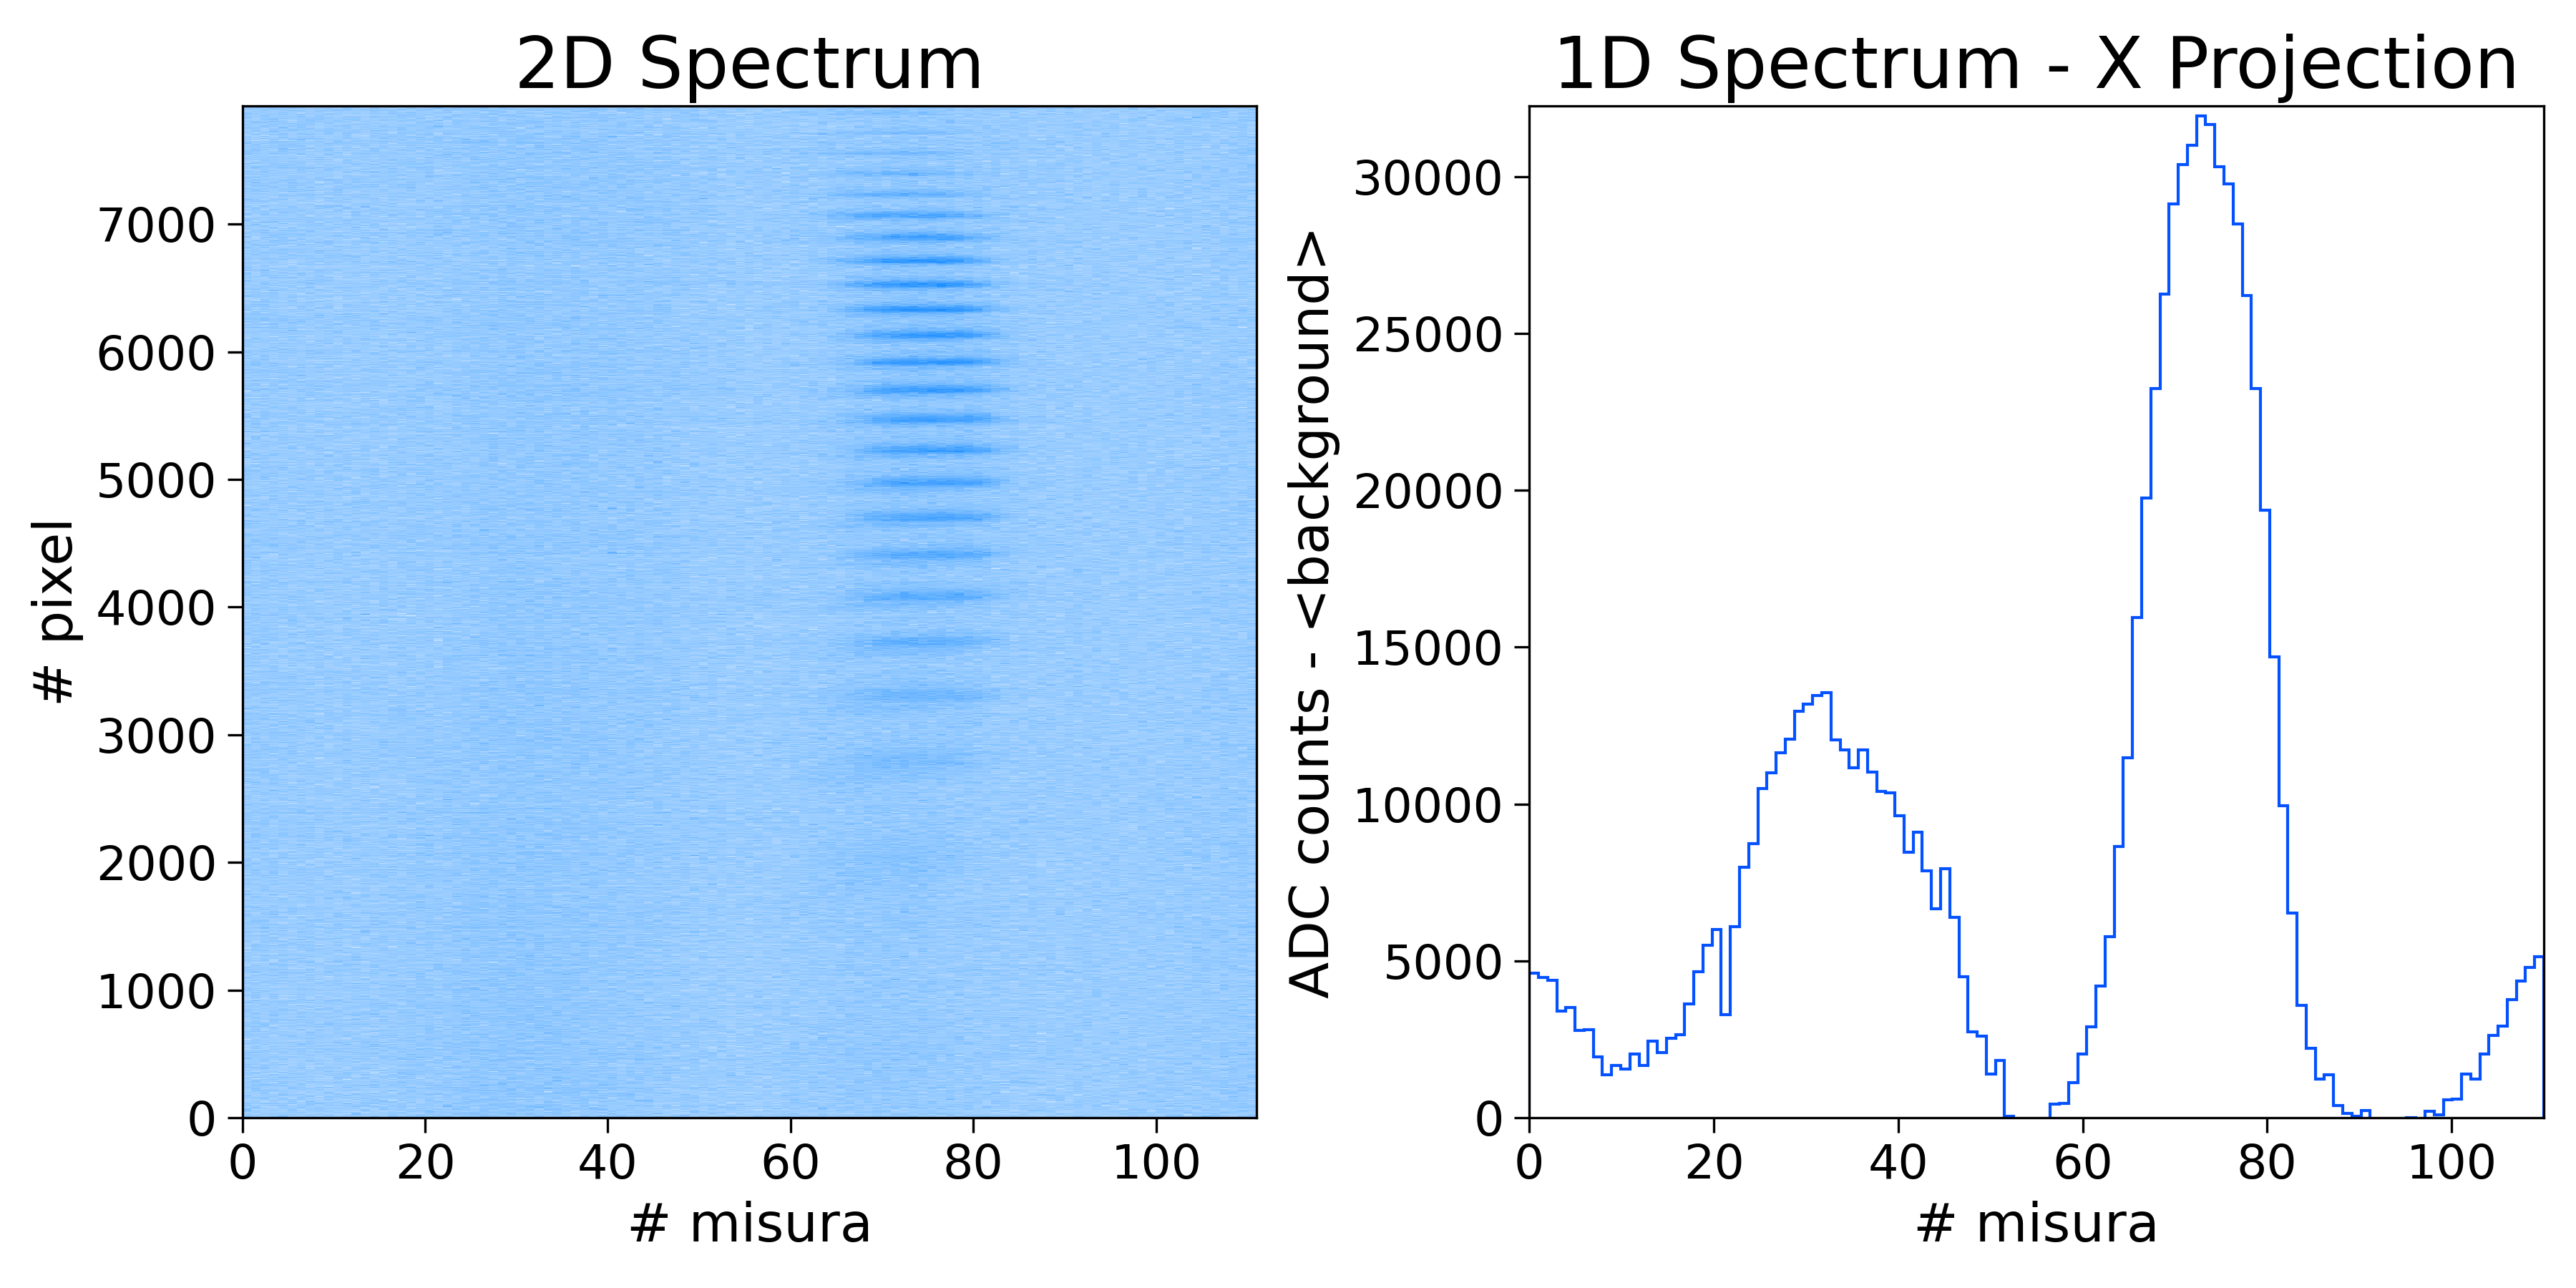
\includegraphics[width=\linewidth]{../Plots/Boff_2d_spectrum.png}
    \caption{Spettro bidimensionale $\text{B}_{\text{off}}$ (a sinistra) e proiezione sull'asse orizzontale (a destra)}
    \label{i:spettro2d_Boff}
\end{figure}

% \begin{figure}
%     \centering
%     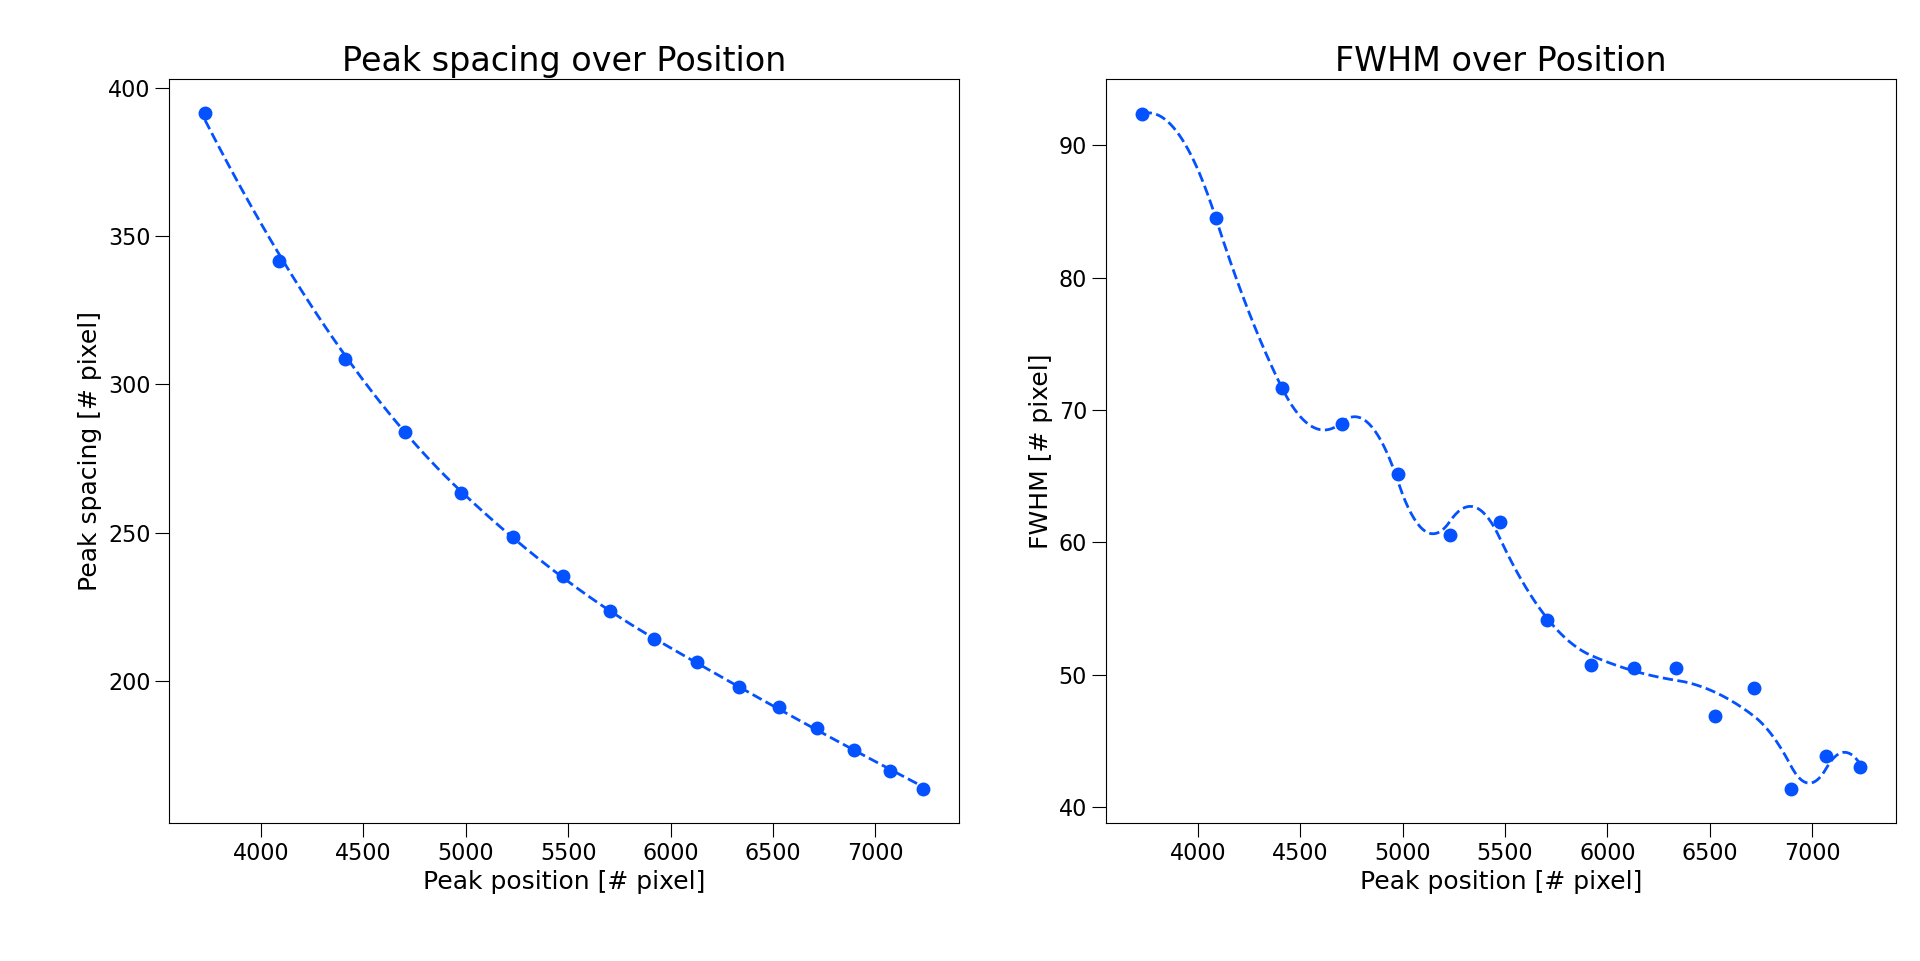
\includegraphics[width=\linewidth]{../Plots/Boff_spacing_trend.png}
%     \caption{Spacing trend}
%     \label{i:spacing_trend_Boff}
% \end{figure}

% QUESTO SERVE PER METTERE DUE FIGURE PICCOLE UNA AFFIANCO ALL'ALTRA
% \begin{figure*}[htp]
%     \centering
%     \subfigure[Spettro bidimensionale $\text{B}_{\text{off}}$]{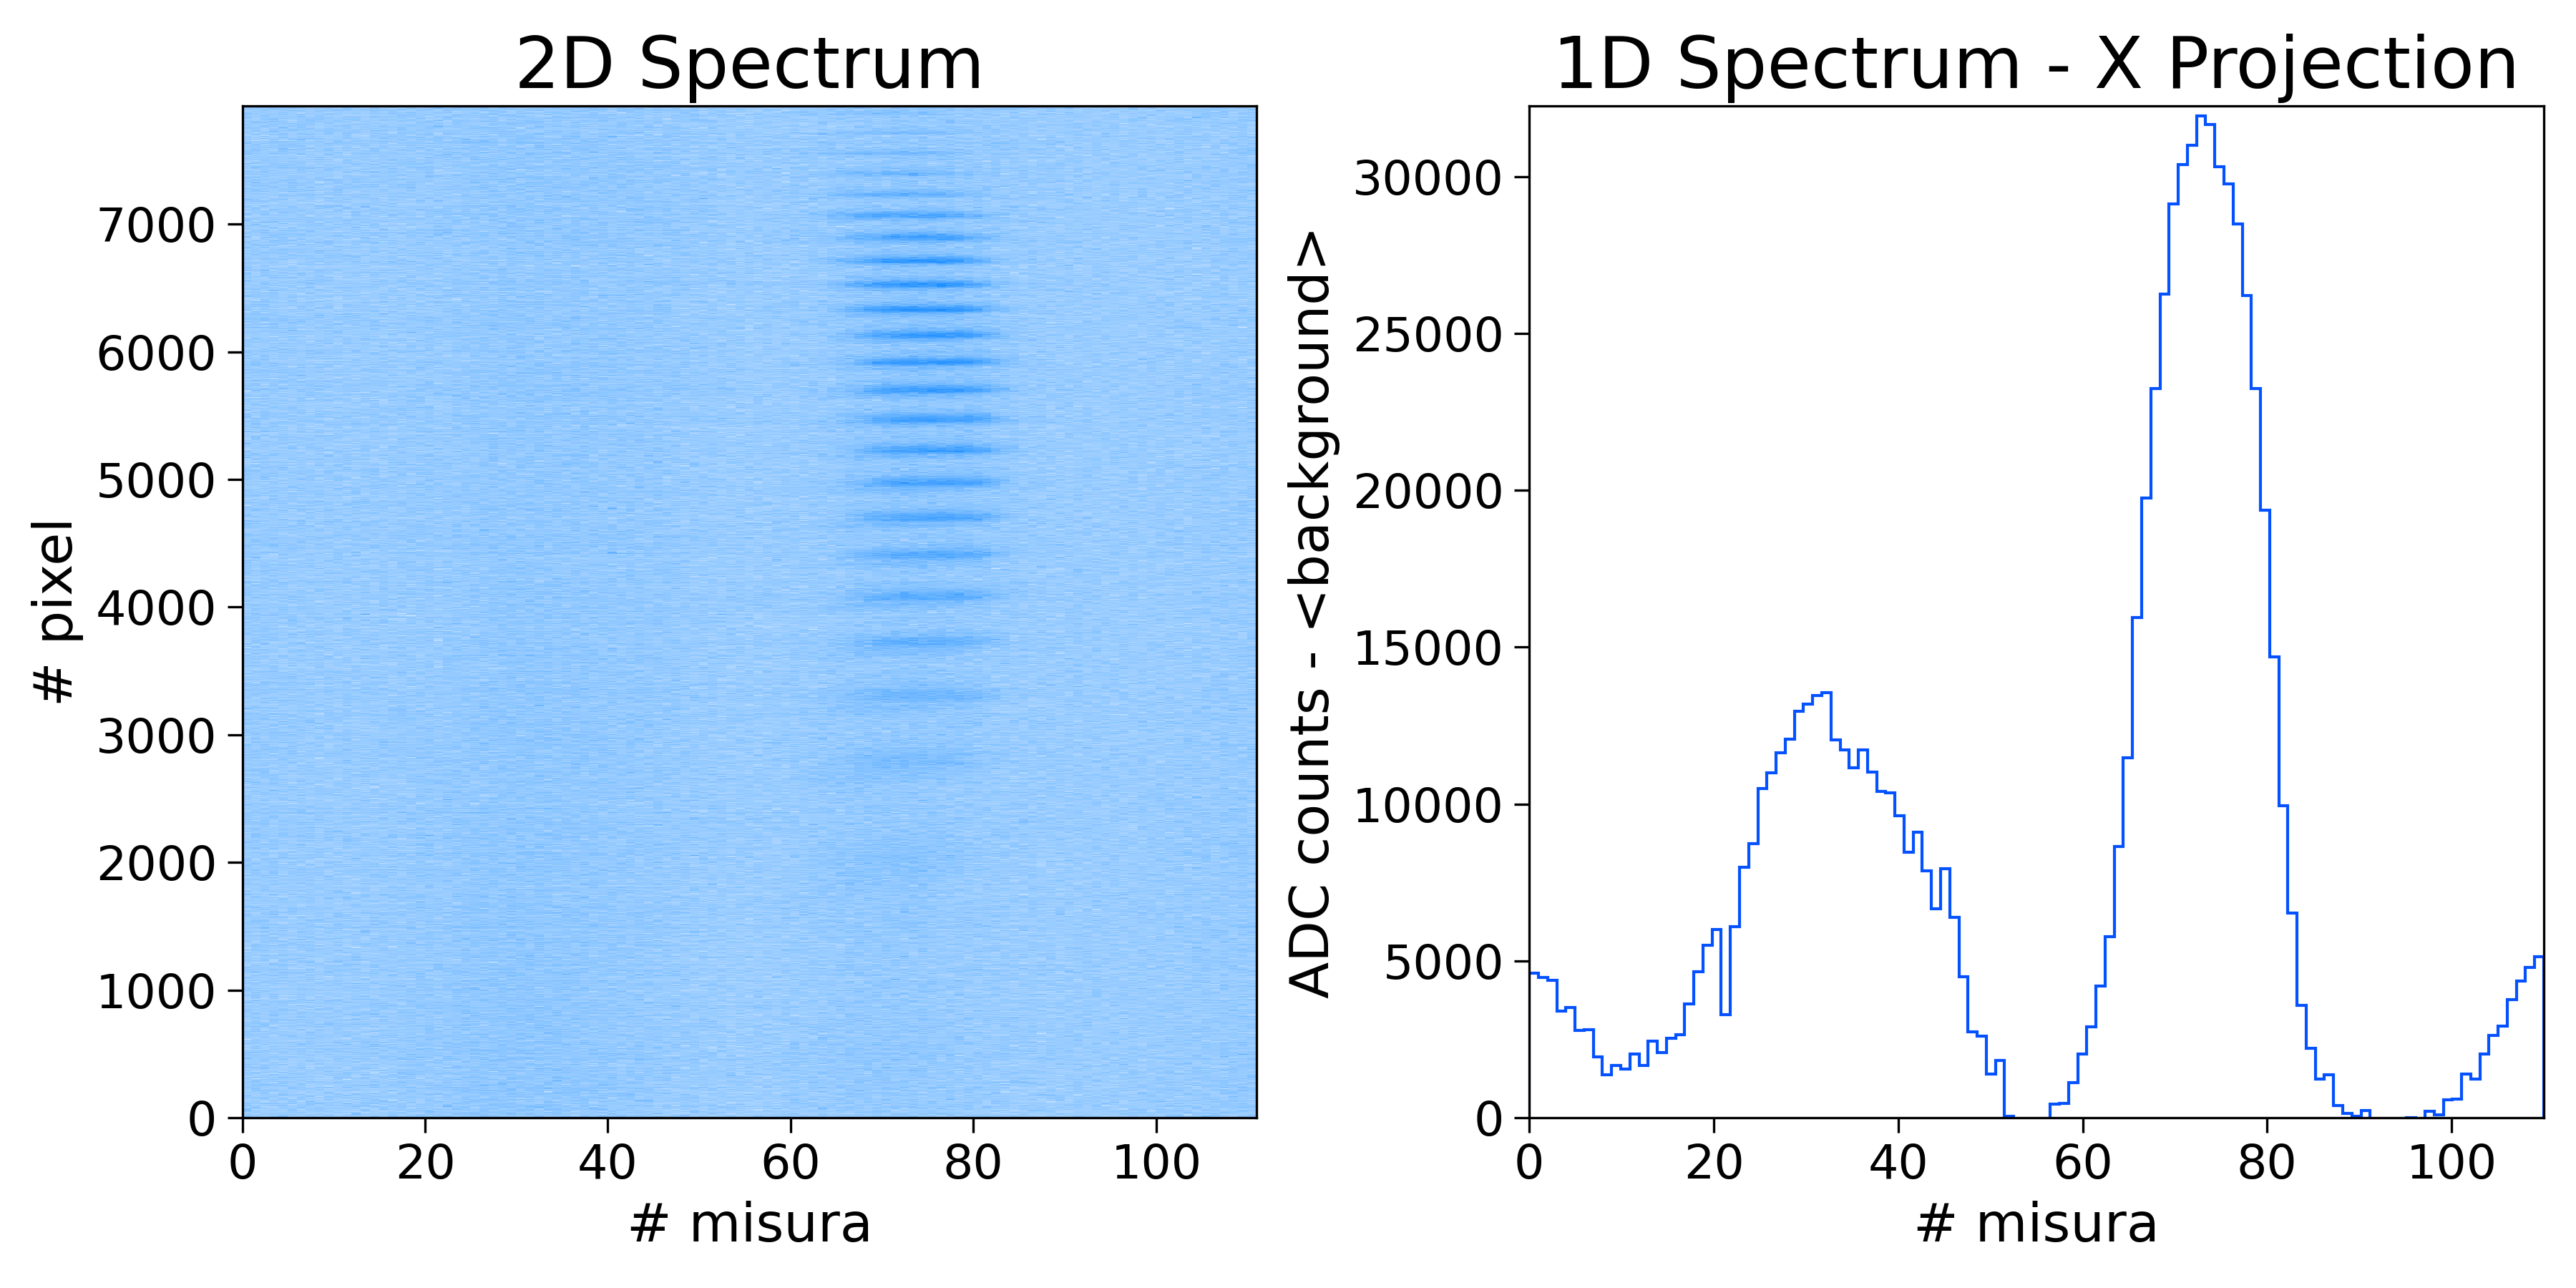
\includegraphics[width=0.5\textwidth]{../Plots/Boff_2d_spectrum.png}}\label{i:spettro2d_Boff}\hfill
%     \subfigure[Spacing trend]{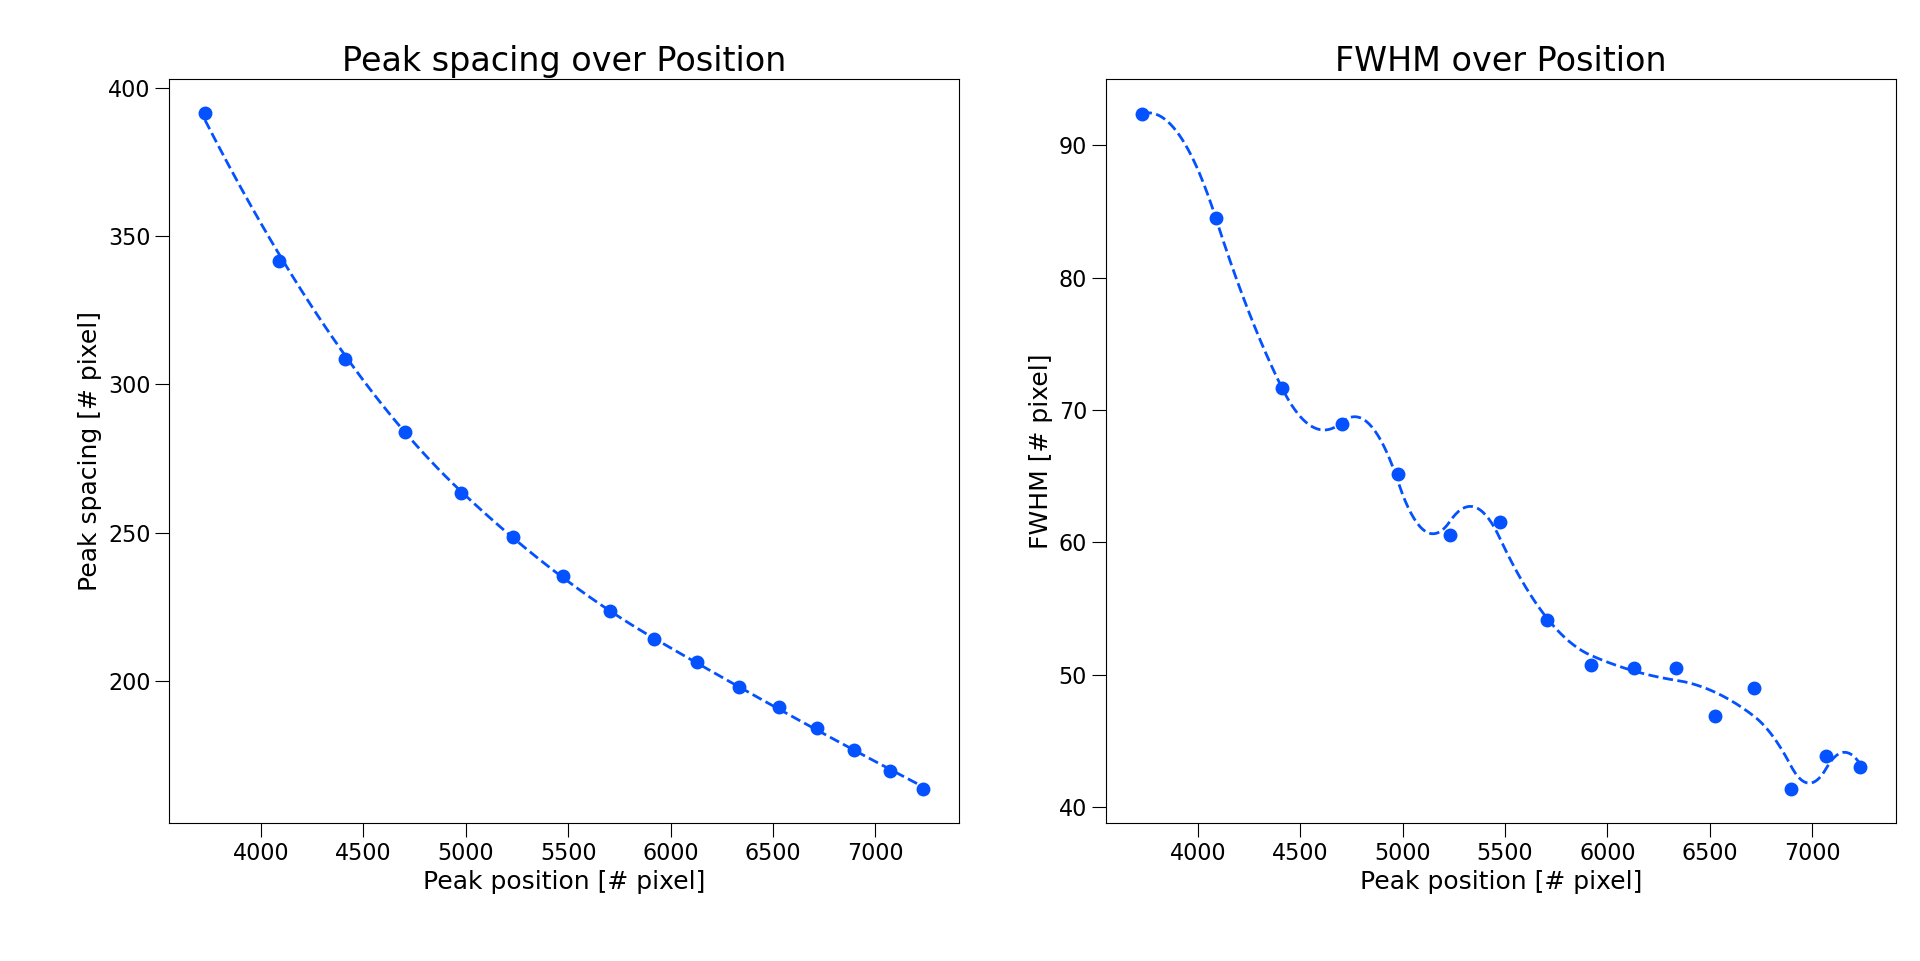
\includegraphics[width=0.5\textwidth]{../Plots/Boff_spacing_trend.png}}\label{i:spacing_trend_Boff}
%   \end{figure*}

 \begin{figure*}
     \centering
     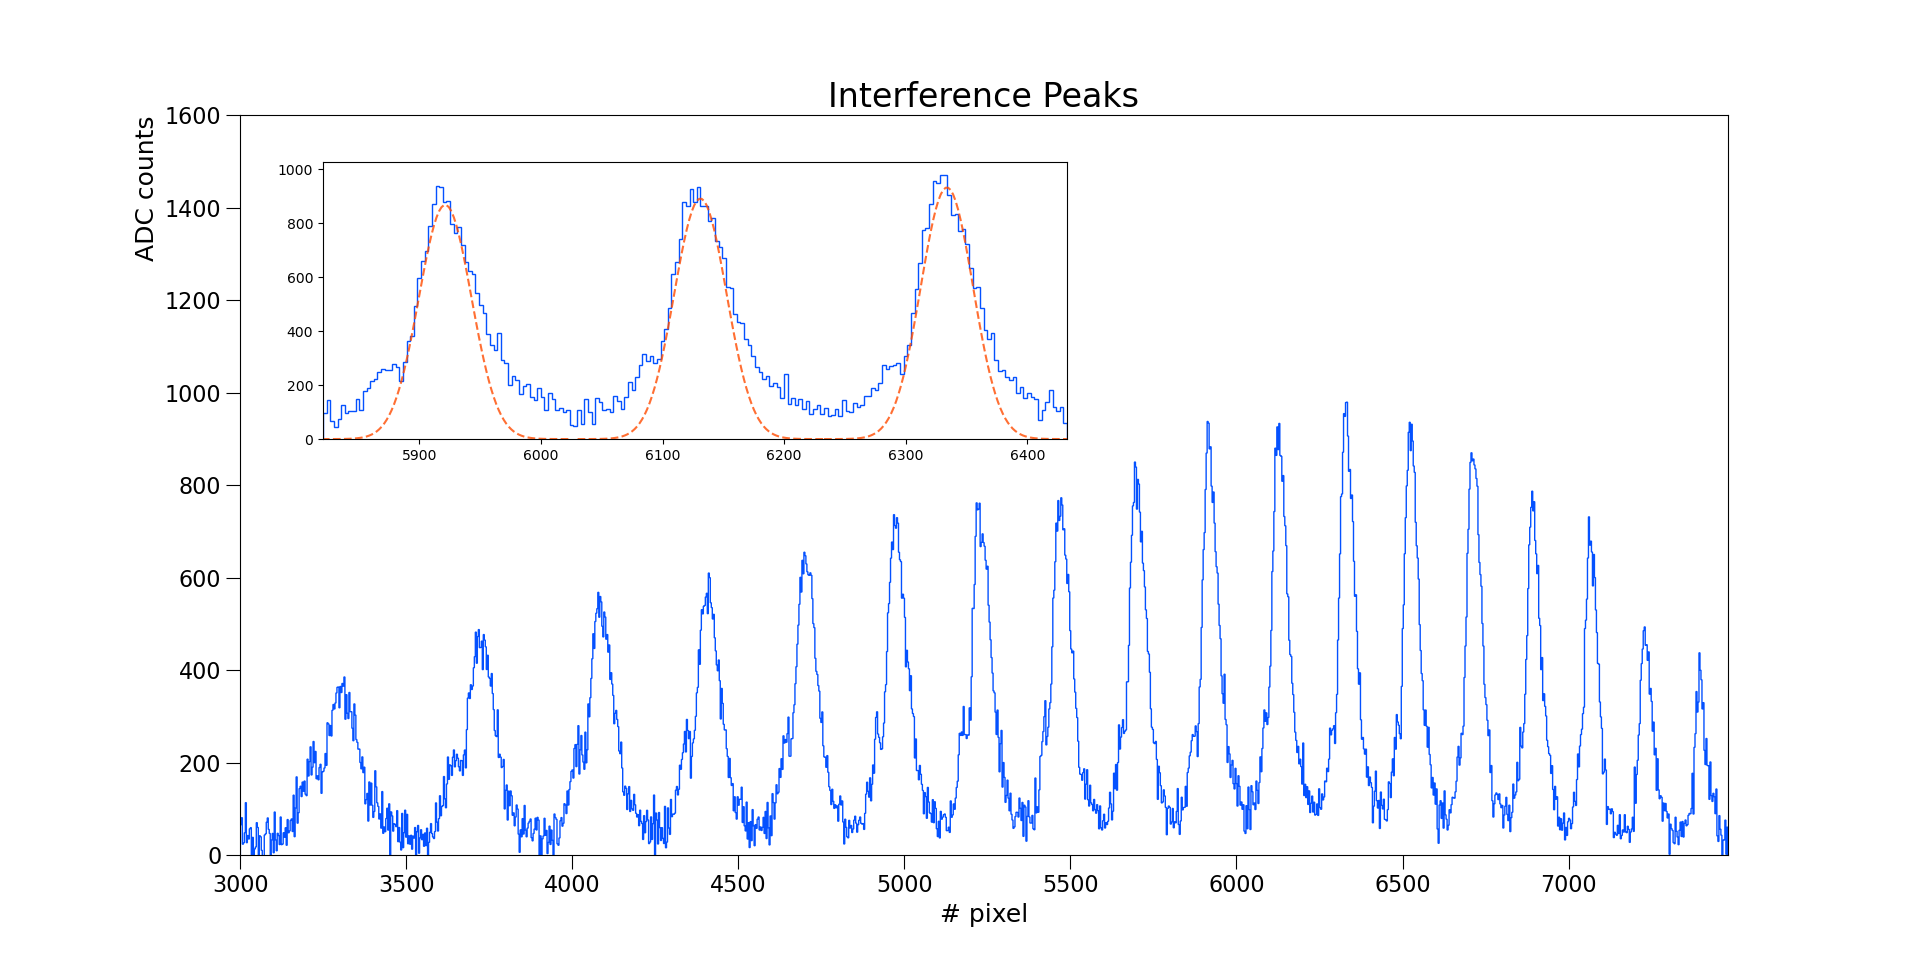
\includegraphics[width=\textwidth]{../Plots/Boff_Y_proj.png}
    \caption{Proiezione sull'asse y dello spettro bidimensionale $\text{B}_{\text{off}}$}
     \label{i:spettro2d_Boff_ProjY}
 \end{figure*}




\cleardoublepage
% %%%%%%%%%%%%%%%%%%%%%%%%%%%%%%%%%%%%%%%%%%%%%%%%%%%%%%%%%%%%%%%%%%%%%%
\section{Fattore di Landè}\label{s:lande}

% \begin{itemize}
%     \item Lo calcoliamo con Bon lungo la direzione della radiazione (parlare dello splitting di Zeeman)
%     \item Formule (range utile + conversione energia + fattore di Landè)
%     \item Procedura di analisi (niente fit perchè non vengono)
%     \item Plot con tutti i picchi + finestrella con lo zoom su una tripletta 
%     \item Controllare che lo splitting Zeeman non subisca aberrazione pesante
% \end{itemize}
Il fattore di Landè si ricava dalla relazione: 

\vspace{-15pt}
\begin{equation}
    \text{g}_{\text{L}} = - \frac{\Delta \text{E}_{\text{zee}}}{\mu_{\text{B}} \text{m}_{\text{j}} \text{B} }
    \label{e:gL}
\vspace{-5pt}
\end{equation}
dove $\mu_{\text{B}}$ è il magnetone di Bohr. \\
Si analizzano i dati con il campo magnetico acceso e osservando la radiazione parallelamente a
$\vec{\text{B}}$. Poiché un dipolo non emette lungo la direzione che individua, i termini polarizzati circolarmente
corrispondenti a $\Delta \text{m} = \pm 1$ hanno intensità maggiore dei termini corrispondenti a $\Delta \text{m} = 0$.
Perciò la transizione centrale è soppressa e si osservano solo le due laterali, separate da $\delta\lambda = 2
\Delta\lambda_{\text{zee}}$, dove $\Delta\lambda_{\text{zee}}$ rappresenta lo splitting Zeeman. La presenza del 
campo magnetico induce una separazione energetica pari a 

\vspace{-15pt}
\begin{equation}
    \Delta \text{E}_{\text{zee}} = \frac{\text{hc}}{\lambda^2} \cdot \Delta\lambda_{\text{zee}}
    \label{e:dEzee}
\vspace{-5pt}
\end{equation}


% \begin{figure*}
%     \centering
%     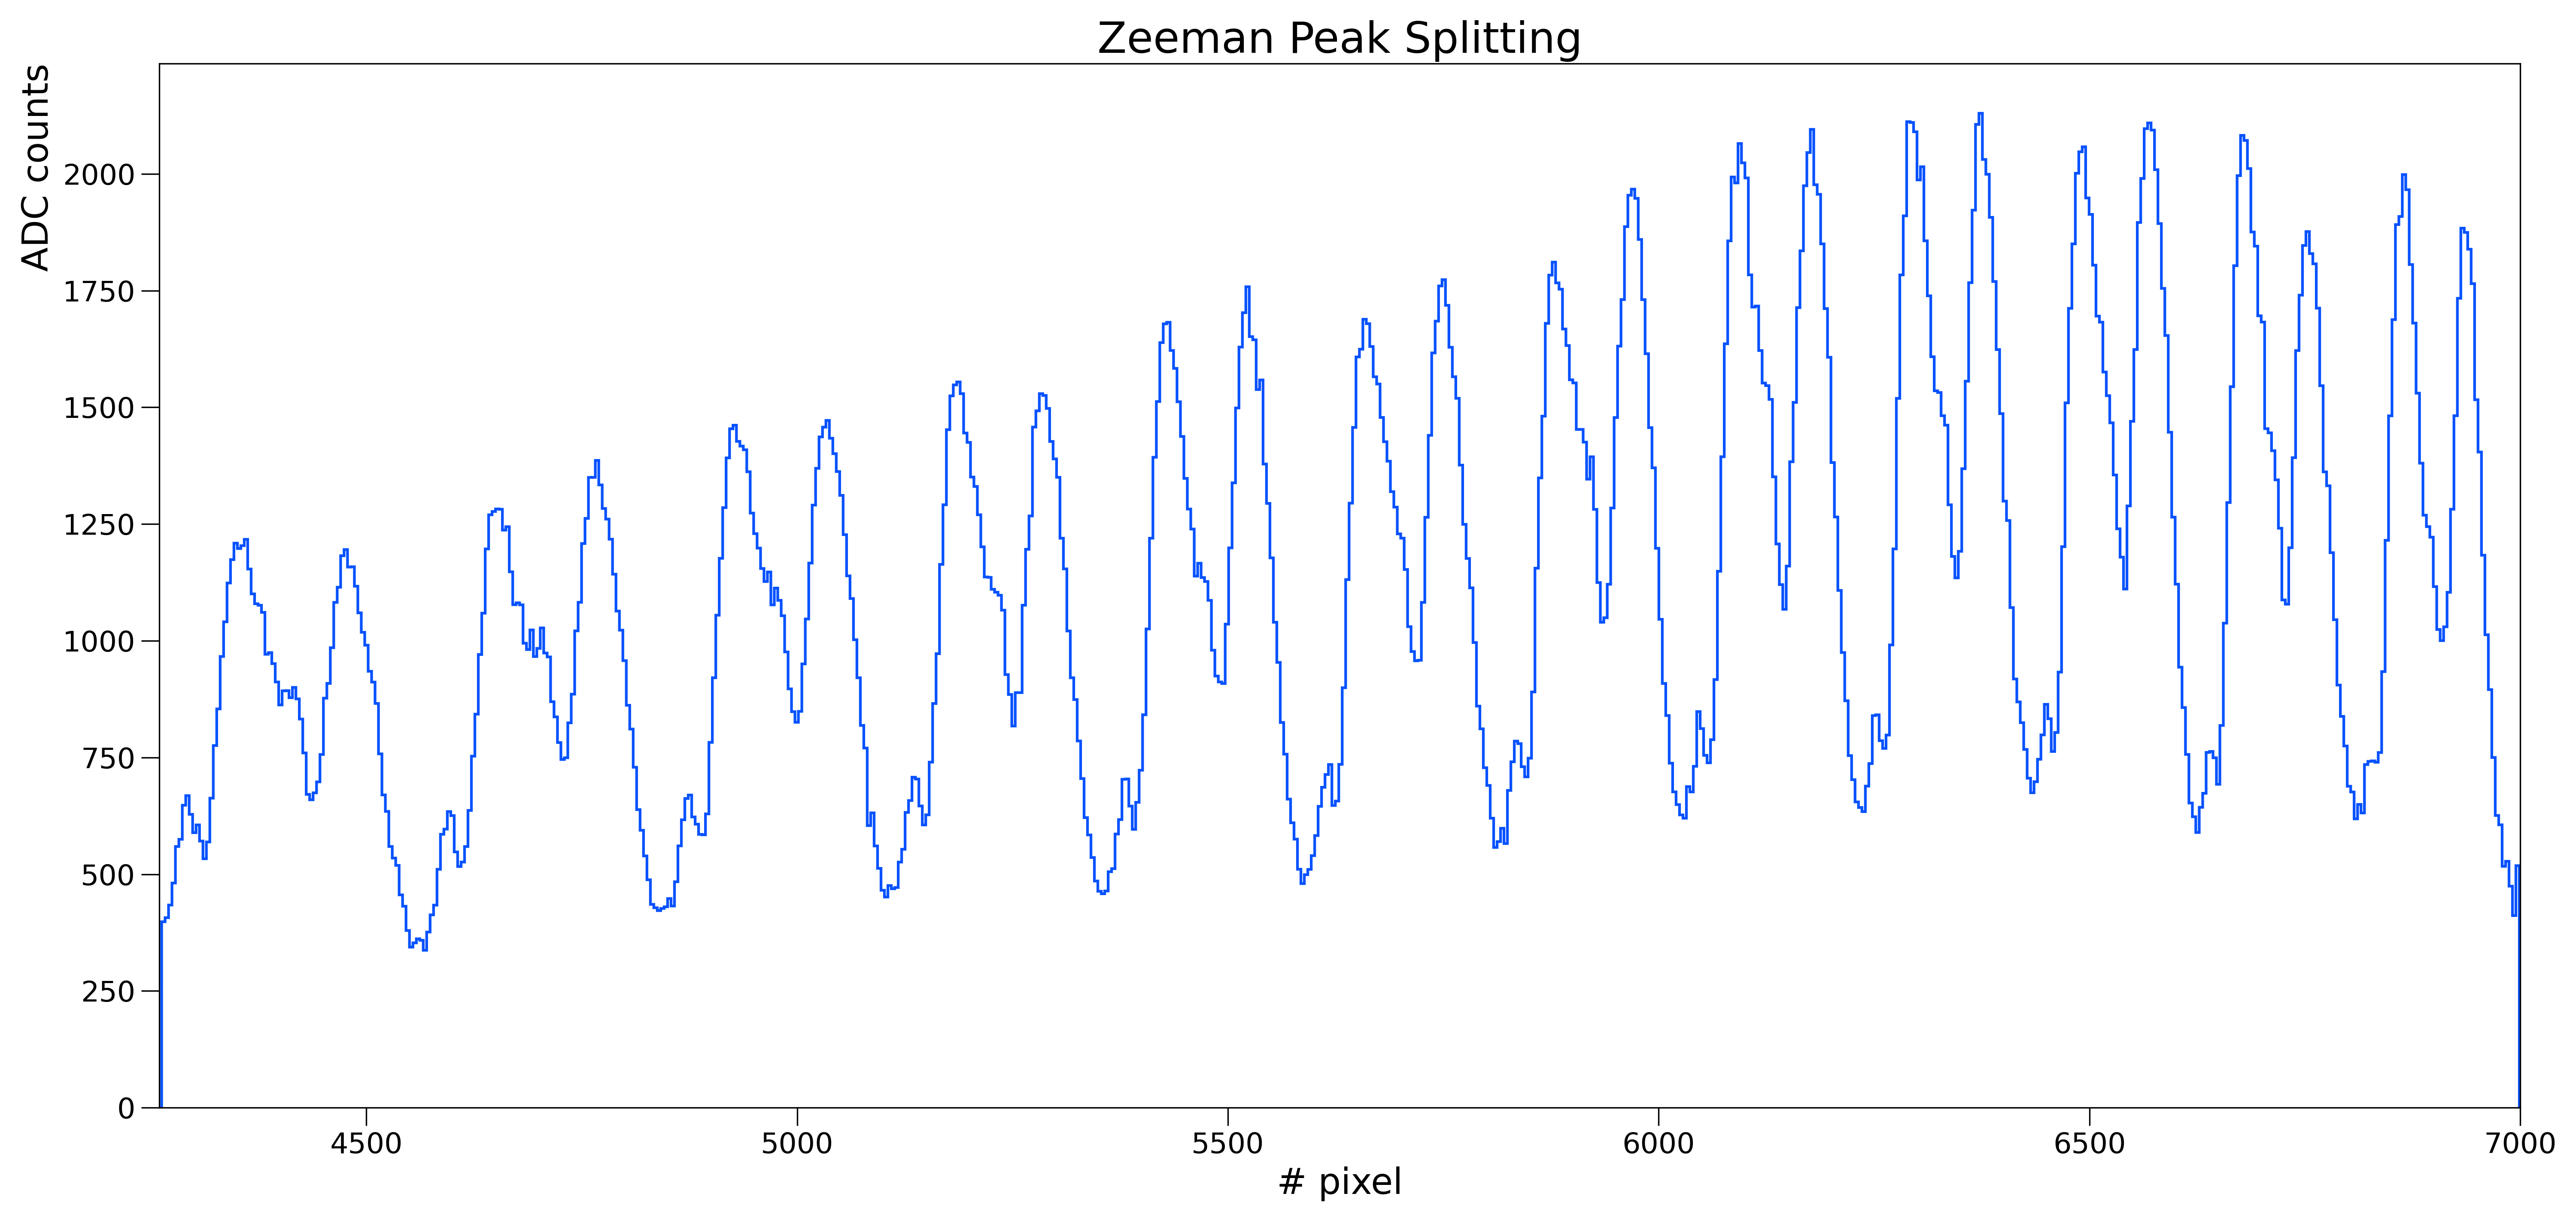
\includegraphics[width=\textwidth]{../Plots/Bon_Y_proj.png}
%     \caption{Proiezione sull'asse y $\text{B}_{on}$}
%     \label{i:spettro2d_Bon_ProjY}
% \end{figure*}

% \begin{figure}[h]
%     \centering
%     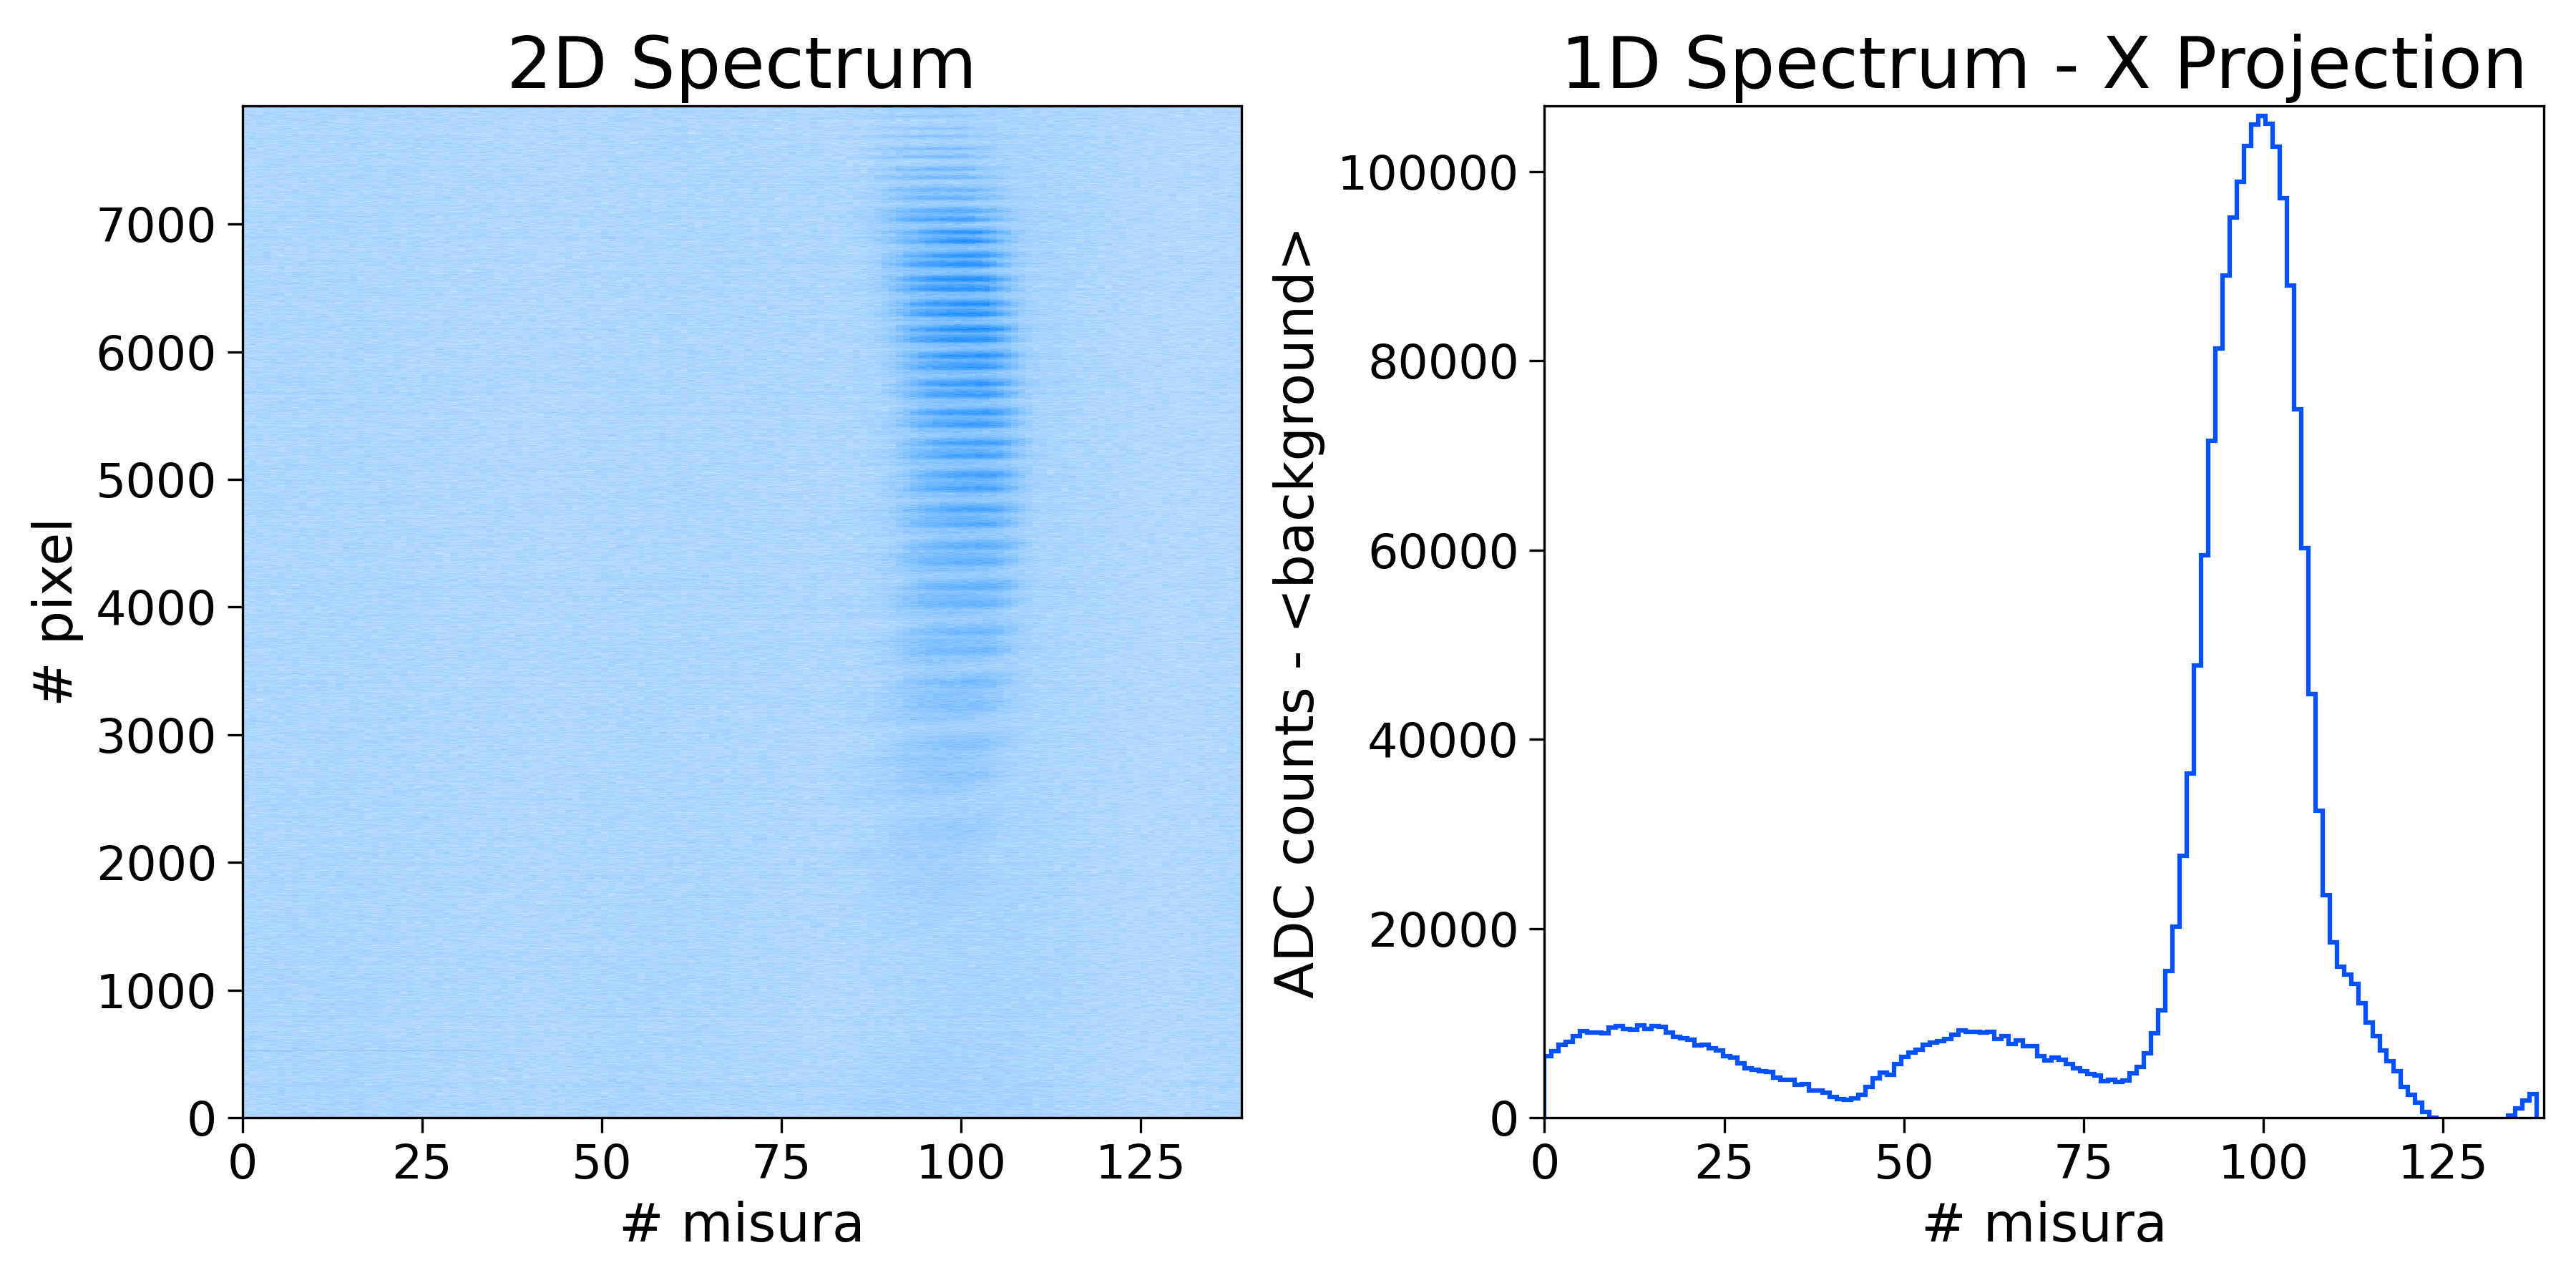
\includegraphics[width=\linewidth]{../Plots/Bon_2d_spectrum.png}
%     \caption{Spettro bidimensionale $\text{B}_{on}$}
%     \label{i:spettro2d_Bon}
% \end{figure}




% %%%%%%%%%%%%%%%%%%%%%%%%%%%%%%%%%%%%%%%%%%%%%%%%%%%%%%%%%%%%%%%%%%%%%%
\section{Campo magnetico ortogonale alla radiazione}\label{s:ortogonale}

% \begin{figure*}
%     \centering
%     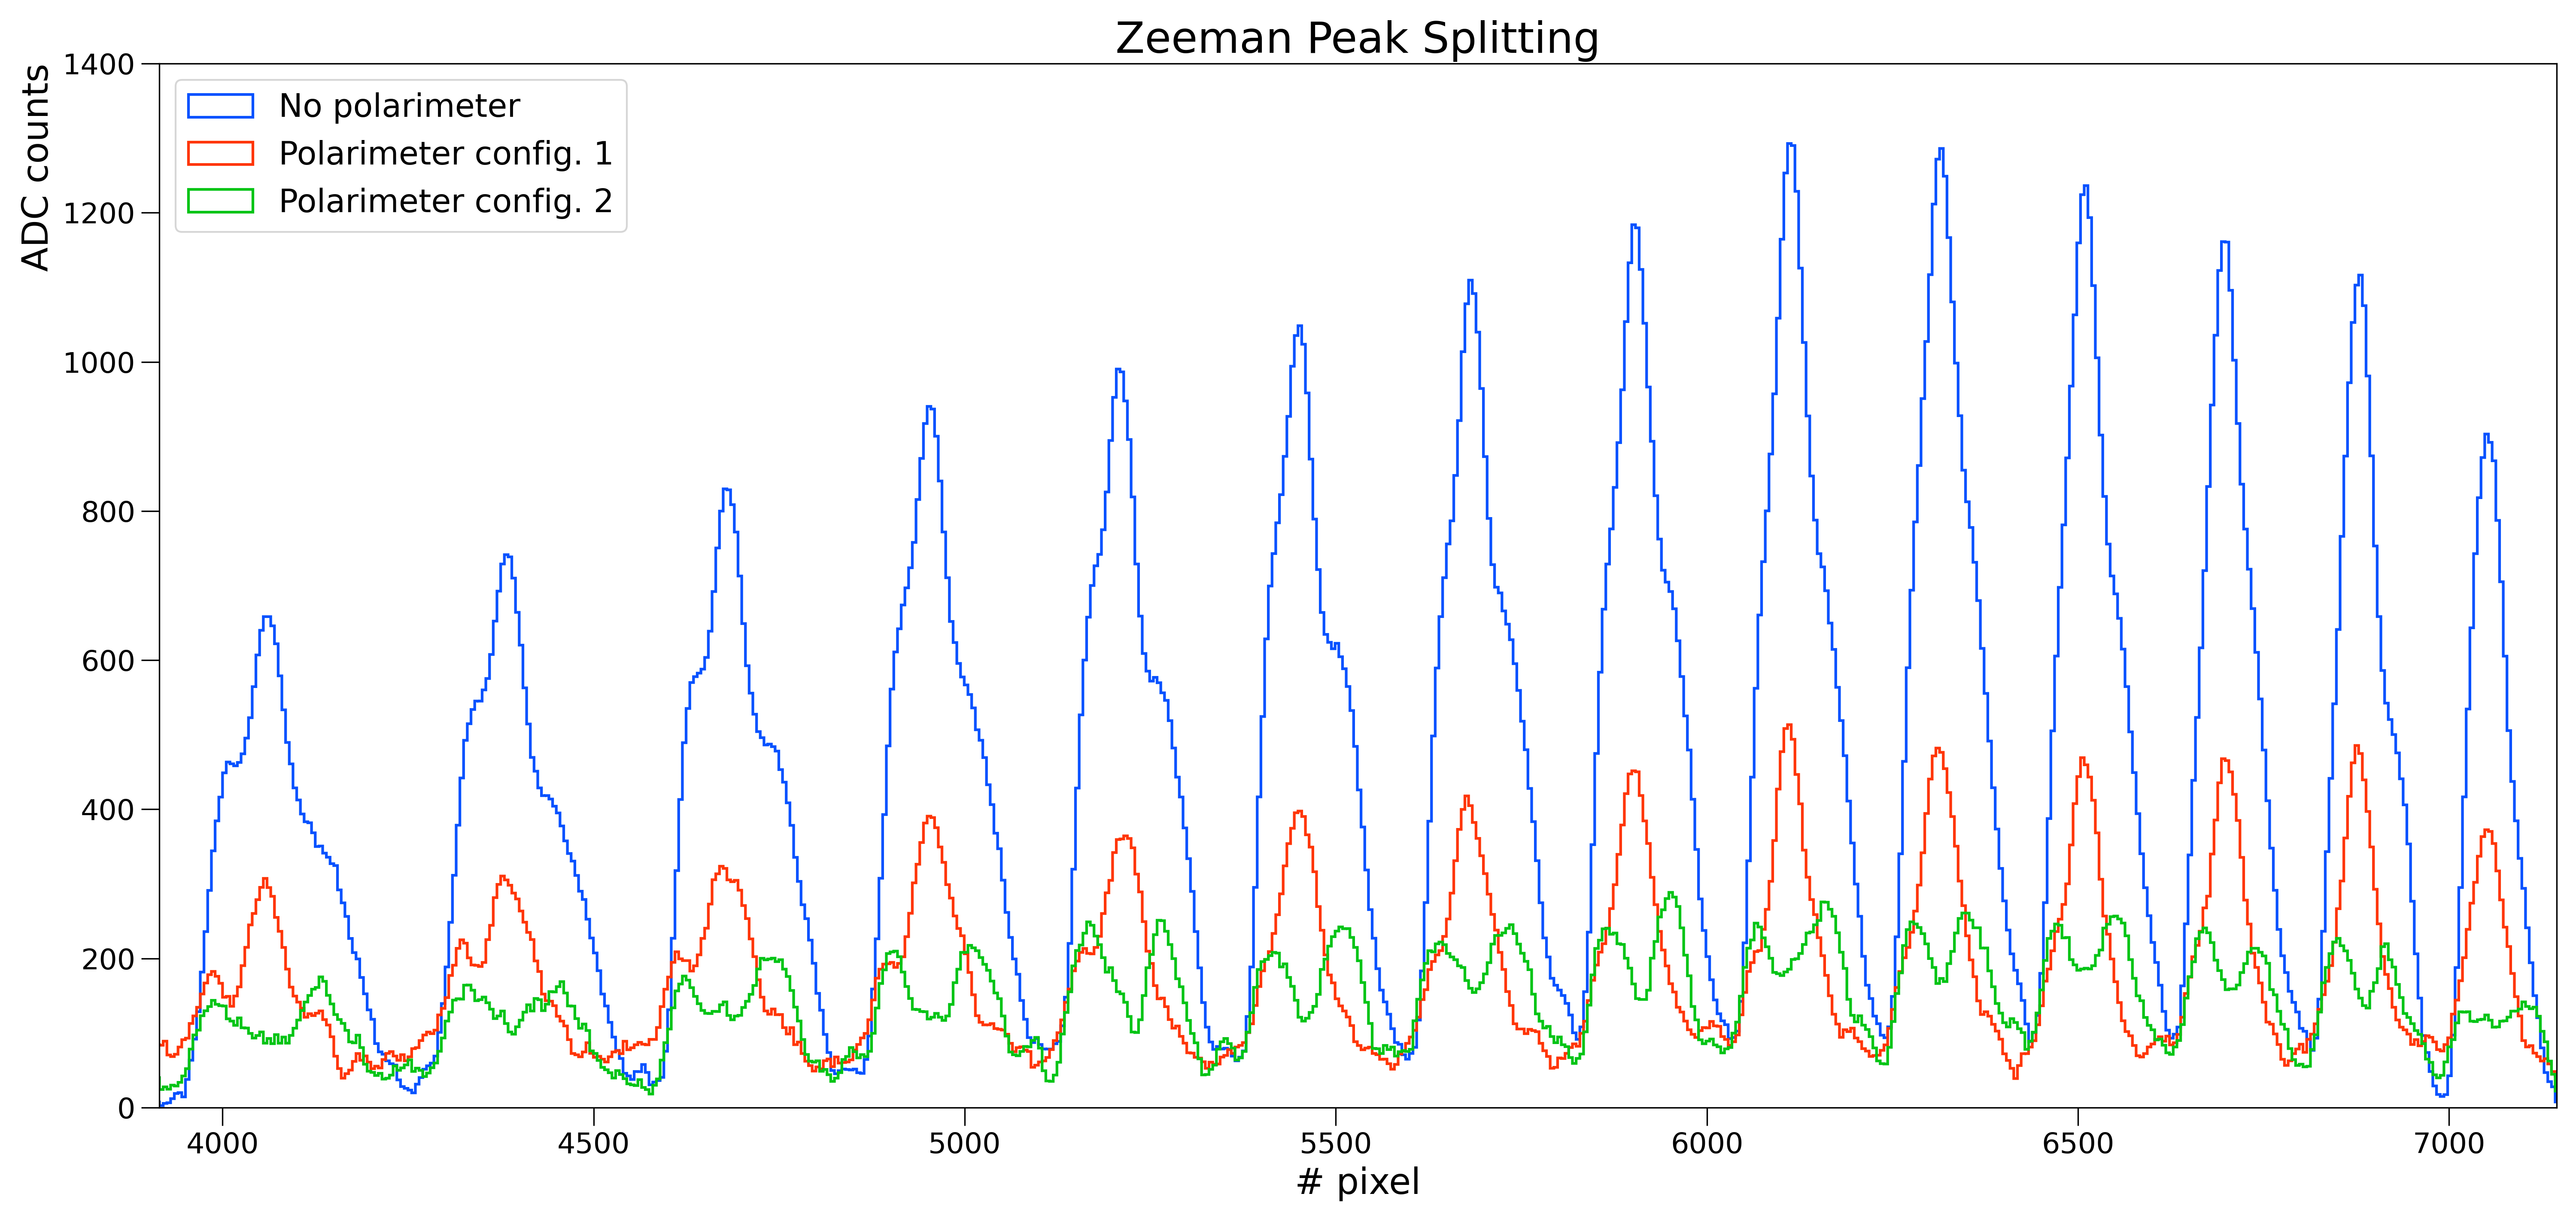
\includegraphics[width=\textwidth]{../Plots/Bon_overlap_big.png}
%     \caption{Proiezione sull'asse y dello spettro bidimensionale nelle configurazioni con e senza polarizzatore}
%     \label{i:spettro2d_overlap}
% \end{figure*}

% \begin{itemize}
%     \item Un po' di fisica più in dettaglio rispetto all'introduzione (polarizzazione ecc) + aspettative "teoriche"
%     (intensità picchi ecc)
%     \item Plot istogrammi sovrapposti 
%     \item Deduzione configurazioni polarimetro dal plot 
% \end{itemize}

Si analizzano i dati acquisiti ruotando il campo magnetico, cioè osservando la radiazione emessa in direzione ortogonale
a $\vec{\text{B}}$. In questo caso, i termini associati a $\Delta \text{m} = 0$ presentano polarizzazione lineare,
mentre quelli relativi a $\Delta \text{m} = \pm 1$ sono polarizzati circolarmente in senso orario o antiorario. Ci si
aspetta quindi di osservare un tripletto, cioè la formazione di tre righe equispaziate visibili nella direzione di
propagazione trasversa al campo. Successivamente, si inserisce un filtro polarizzatore di fronte alla lente condensante,
che viene impiegato in due configurazioni, non note a priori. Se il polarizzatore fa passare prevalentemente la
componente della luce polarizzata parallelamente alla direzione del campo, allora si osserva una sola riga; se invece,
ruotando il filtro, questo fa passare la componente della luce con polarizzazione ortogonale al campo, allora la
transizione centrale viene soppressa e si osservano solamente i due picchi laterali. Conseguentemente ci si aspetta che
l'intensità della radiazione sia significativamente ridotta con l'inserimento del filtro polarizzatore.  
In \autoref{i:spettro2d_overlap} è riportata la proiezione sull'asse y dello spettro bidimensionale, nelle tre
configurazioni precedentamente descritte. Si nota che, in generale, l'apparato non permette di risolvere
sufficientemente bene le transizioni: questo è particolarmente evidente in assenza del filtro, in quanto non è possibile
distinguere i tre picchi di interferenza distinti che ci si aspetterebbe. Inoltre, si osserva che nella prima
configurazione lo spettro è caratterizzato dalla presenza di un unico picco, mentre nella seconda da un doppietto: da
ciò si deduce che nel primo caso il polarizzatore è posto lungo la direzione del campo, mentre nella seconda è ruotato
di 90 gradi. 

\end{document}
